Perhaps the most straighforward question in this paper.

\begin{parts}
	\part From the question we have:
	\begin{equation*}
		\mathbf{j}_\textnormal{h} = -\underbracket{\kappa}_{\kappa_{ij}} \bm{\nabla} T
	\end{equation*}
	
	We also know the tensor transformation law:
	\begin{equation*}
		\kappa_{ij}^\prime = \pderi{x_i^\prime}{x_a} \pderi{x_j^\prime}{x_b} \kappa_{ab}
	\end{equation*}
	
	By Neumann's Principle, the bulk properties of a crystal should reflect its symmetries.
	In an orthorhombic crystal, we have symmetry elements $2_x$, $2_y$, $2_z$.
	
	Hence about an axis we have the following 2-fold rotation matrix (about the subspace of its normal plane):
	\begin{gather*}
		\begin{pmatrix}
			-1 & 0 \\
			0 & -1
		\end{pmatrix} \\
		\Rightarrow 2_z = \begin{pmatrix}
			-1 & &  \\
			& -1 & \\
			& & 1
		\end{pmatrix} \textnormal{\hspace{1em}for example}
	\end{gather*}
	
	Now we need the rotated matrix to be invariant $\Rightarrow$ observe that off-diagonal terms have odd parity under a general rotation and must vanish by symmetry.
	
	Hence $\kappa_{ij} = \textnormal{diag}(\kappa_{xx}, \kappa_{yy}, \kappa_{zz})$.
	
	\part Evaluate $\kappa_\mathbf{u}$ as follows:
	\begin{align*}
		\kappa_\mathbf{u} &\equiv \frac{\mathbf{j}_\textnormal{h} \cdot \hat{\mathbf{u}}}{\abs{\nabla T}} \\
		&= \frac{-\kappa \bm{\nabla}T \cdot \hat{\mathbf{u}}}{\abs{\nabla T}} \\
		&= \frac{\sbracket{\kappa \bcancel{\abs{\nabla T}} \hat{\mathbf{u}}} \cdot \hat{\mathbf{u}}}{\bcancel{\abs{\nabla T}}} \\
		&= \begin{pmatrix}
			\kappa_{xx} u_x & \kappa_{yy} u_y & \kappa_{zz} u_z
		\end{pmatrix}
		\begin{pmatrix}
			u_x \\ u_y \\ u_z
		\end{pmatrix} \\
		&= u_x^2 \kappa_{xx} + u_y^2 \kappa_{yy} + u_z^2 \kappa_{zz} \textnormal{\hspace{1em}in orthorhombic crystal}
	\end{align*}
	
	\part We know $a = \SI{0.575}{\nano\metre}$, $b = \SI{0.587}{\nano\metre}$, $c = \SI{0.769}{\nano\metre}$, and that $\widehat{\mathbf{a} + \mathbf{b}} = \dfrac{a \hat{\mathbf{x}} + b \hat{\mathbf{y}}}{\sqrt{a^2 + b^2}}$:
	\begin{align}
		\kappa_{\sbracket{1 1 0}} &= \rbracket{\frac{a}{\sqrt{a^2 + b^2}}}^2 \kappa_{xx} + \rbracket{\frac{b}{\sqrt{a^2 + b^2}}}^2 \kappa_{yy} + 0 \notag \\
		&= \SI{24.2}{\watt\per\metre\per\kelvin} = \frac{a^2 \kappa_{xx} + b^2 \kappa_{yy}}{a^2 + b^2}
		\label{eqn:q6-kappa-110}
	\end{align}
	
	Similarly,
	\begin{align}
		\kappa_{\sbracket{1 \bar{2} 0}} &= \rbracket{\frac{a}{\sqrt{a^2 + 4b^2}}}^2 \kappa_{xx} + \rbracket{\frac{2b}{\sqrt{a^2 + 4b^2}}}^2 \kappa_{yy} + 0 \notag \\
		&= \SI{28.1}{\watt\per\metre\per\kelvin} = \frac{a^2 \kappa_{xx} + 4b^2 \kappa_{yy}}{a^2 + 4b^2}
		\label{eqn:q6-kappa-1-20}
	\end{align}
	\begin{align}
		\kappa_{\sbracket{0 0 1}} &= 0 + 0 + \rbracket{\frac{c}{\sqrt{c^2}}} \kappa_{zz} \notag \\
		&= \SI{5.4}{\watt\per\metre\per\kelvin} = \kappa_{zz}
		\label{eqn:q6-kappa-001}
	\end{align}
	
	Combining \eqref{eqn:q6-kappa-110} and \eqref{eqn:q6-kappa-1-20} gives:
	\begin{align*}
		\kappa_{xx} &= \SI{17.5}{\watt\per\metre\per\kelvin} \\
		\kappa_{yy} &= \SI{30.6}{\watt\per\metre\per\kelvin}
	\end{align*}
	
	\part Momentum transfer triangle in a reciprocal lattice:
	\begin{figure}[H]
		\centering
		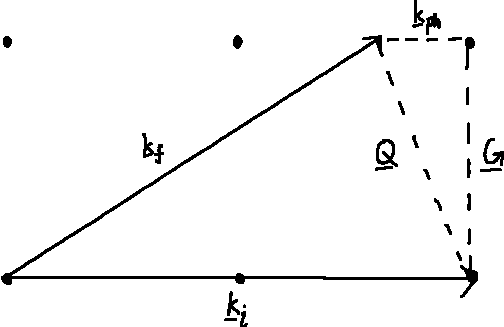
\includegraphics[width=.6\linewidth]{q6-momentum-triangle}
	\end{figure}
	We know that phase velocity $v = \omega / k$ and $\mathbf{Q} = \mathbf{k}_f - \mathbf{k}_i = \mathbf{G} + \mathbf{k}_\textnormal{ph}$ where $\mathbf{k}_\textnormal{ph}$ is a wavevector in the 1st BZ by the periodicity in the reciprocal lattice.
	
	We then find the wavevector of the phonons ($q_1 = 0.13$, $q_2 = 0.10$):
	\begin{align*}
		k_1 &= q_1 \times \frac{2\pi}{a} \\
		&= \SI{1.42e9}{\per\metre} \\
		k_2 &= q_2 \times \frac{2\pi}{b} \\
		&= \SI{1.07e9}{\per\metre}
	\end{align*}
	
	Hence the velocity of sound along each principal axis is ($\omega = 2\pi\rbracket{\SI{1.0e12}{\hertz}} = \SI{6.28e12}{\radian\per\second}$):
	\begin{align*}
		v_1 &= \frac{\omega}{k_1} \\
		&= \SI{4420}{\metre\per\second} \\
		v_2 &= \frac{\omega}{k_2} \\
		&= \SI{5870}{\metre\per\second}
	\end{align*}
	
	Note that phonon propagation has an anisotropy in the $ab$ plane, since thermal conduction in a solid largely stems from phonon propagation, this physically leads to the anisotropy in heat conduction.
	Also larger $v$ $\rightarrow$ larger $\kappa$.
\end{parts}